\section{Part 1B: Finding and measuring acoustic correlates of stop consonants}

\subsection{Overview}

In the first part of this lab, you explored the spectrographic representation of different vowels of English. Remember that the driving force behind this was the idea that our "one--to--one mapping" hypothesis about speech perception was worth exploring. In other words, we were exploring the idea that there are pieces of acoustic information that are reliably and univocally associated with segmental representations ($=$vowels and consonants). We started with vowels because in a way they are the ``simplest'' case of speech sounds.

You should think about what the first part of the lab has taught you. As far as vowels are concerned, do you think  that the ``one--to--one'' mapping hypothesis is plausible? Do you think the consonant data we will analyze will be consistent or inconsistent with what we have seen for vowels so far?

By now you already know how to\begin{inparaenum}[(a)]~\item produce a spectrogram, \item identify and extract formant information from a spectrogram, \item plot data in \Praat{}\end{inparaenum}. Therefore, the instructions from now on are going to be less detailed.

Now we will proceed to the logical extension of our hypothesis testing, i.e., we will be looking for acoustic correlates of stop consonants in English.The stop consonants we will be looking at are [p b t d k g]. This is the full inventory of stop consonants in English. Stop consonants receive that name because they are basically a full obstruction of the air flow, produced by either the closure of lips ([p b]), the touch of the tip of the tongue against the alveolar ridge ([t d]) or the touch of the back of the tongue against the velum ([k g]). The place where the flow of air is interrupted is called the \emph{place of articulation} of the consonant.

\subsection{Acoustic correlates of place of articulation in stop consonants}

\subsubsection{Before you start}

As you have probably realized by now, formants can be very visible or hard to see, depending on the vowels and the quality of the recording. In this part of the lab, you will be looking at full syllables. As you are going to realize, the shape of the formants seems to be an important piece of information about consonants. However, you can only analyze their shape if you can see them, right? In general, \Praat{}'s automatic formant tracking helps identifying the relevant formants, but here we will be analyzing high quality synthetic syllables created by \citeA{stephens2011}, and the formants should be quite visible in the spectrograms without the automatic formant tracking from \Praat{}. Therefore, I strongly suggest that you turn the formant tracking off before you start analyzing the sound files in this part of the lab. You can click on \softmenu{Formants} $>$ \softmenu{Show formants} and deselect this option.

\subsubsection{aba ada aga}

Load the file \emph{aba\_ada\_aga.wav} in \Praat{}. Once the file is loaded, select it on the \softmenu{Objects} window and then, open the \softmenu{View \& Edit} window. It should look like figure~\ref{step1triplet}:

\begin{figure}[!tbp]
\caption{\Praat{} -- Spectrograms of \emph{aba ada aga}}
\label{step1triplet}
	\begin{center}
		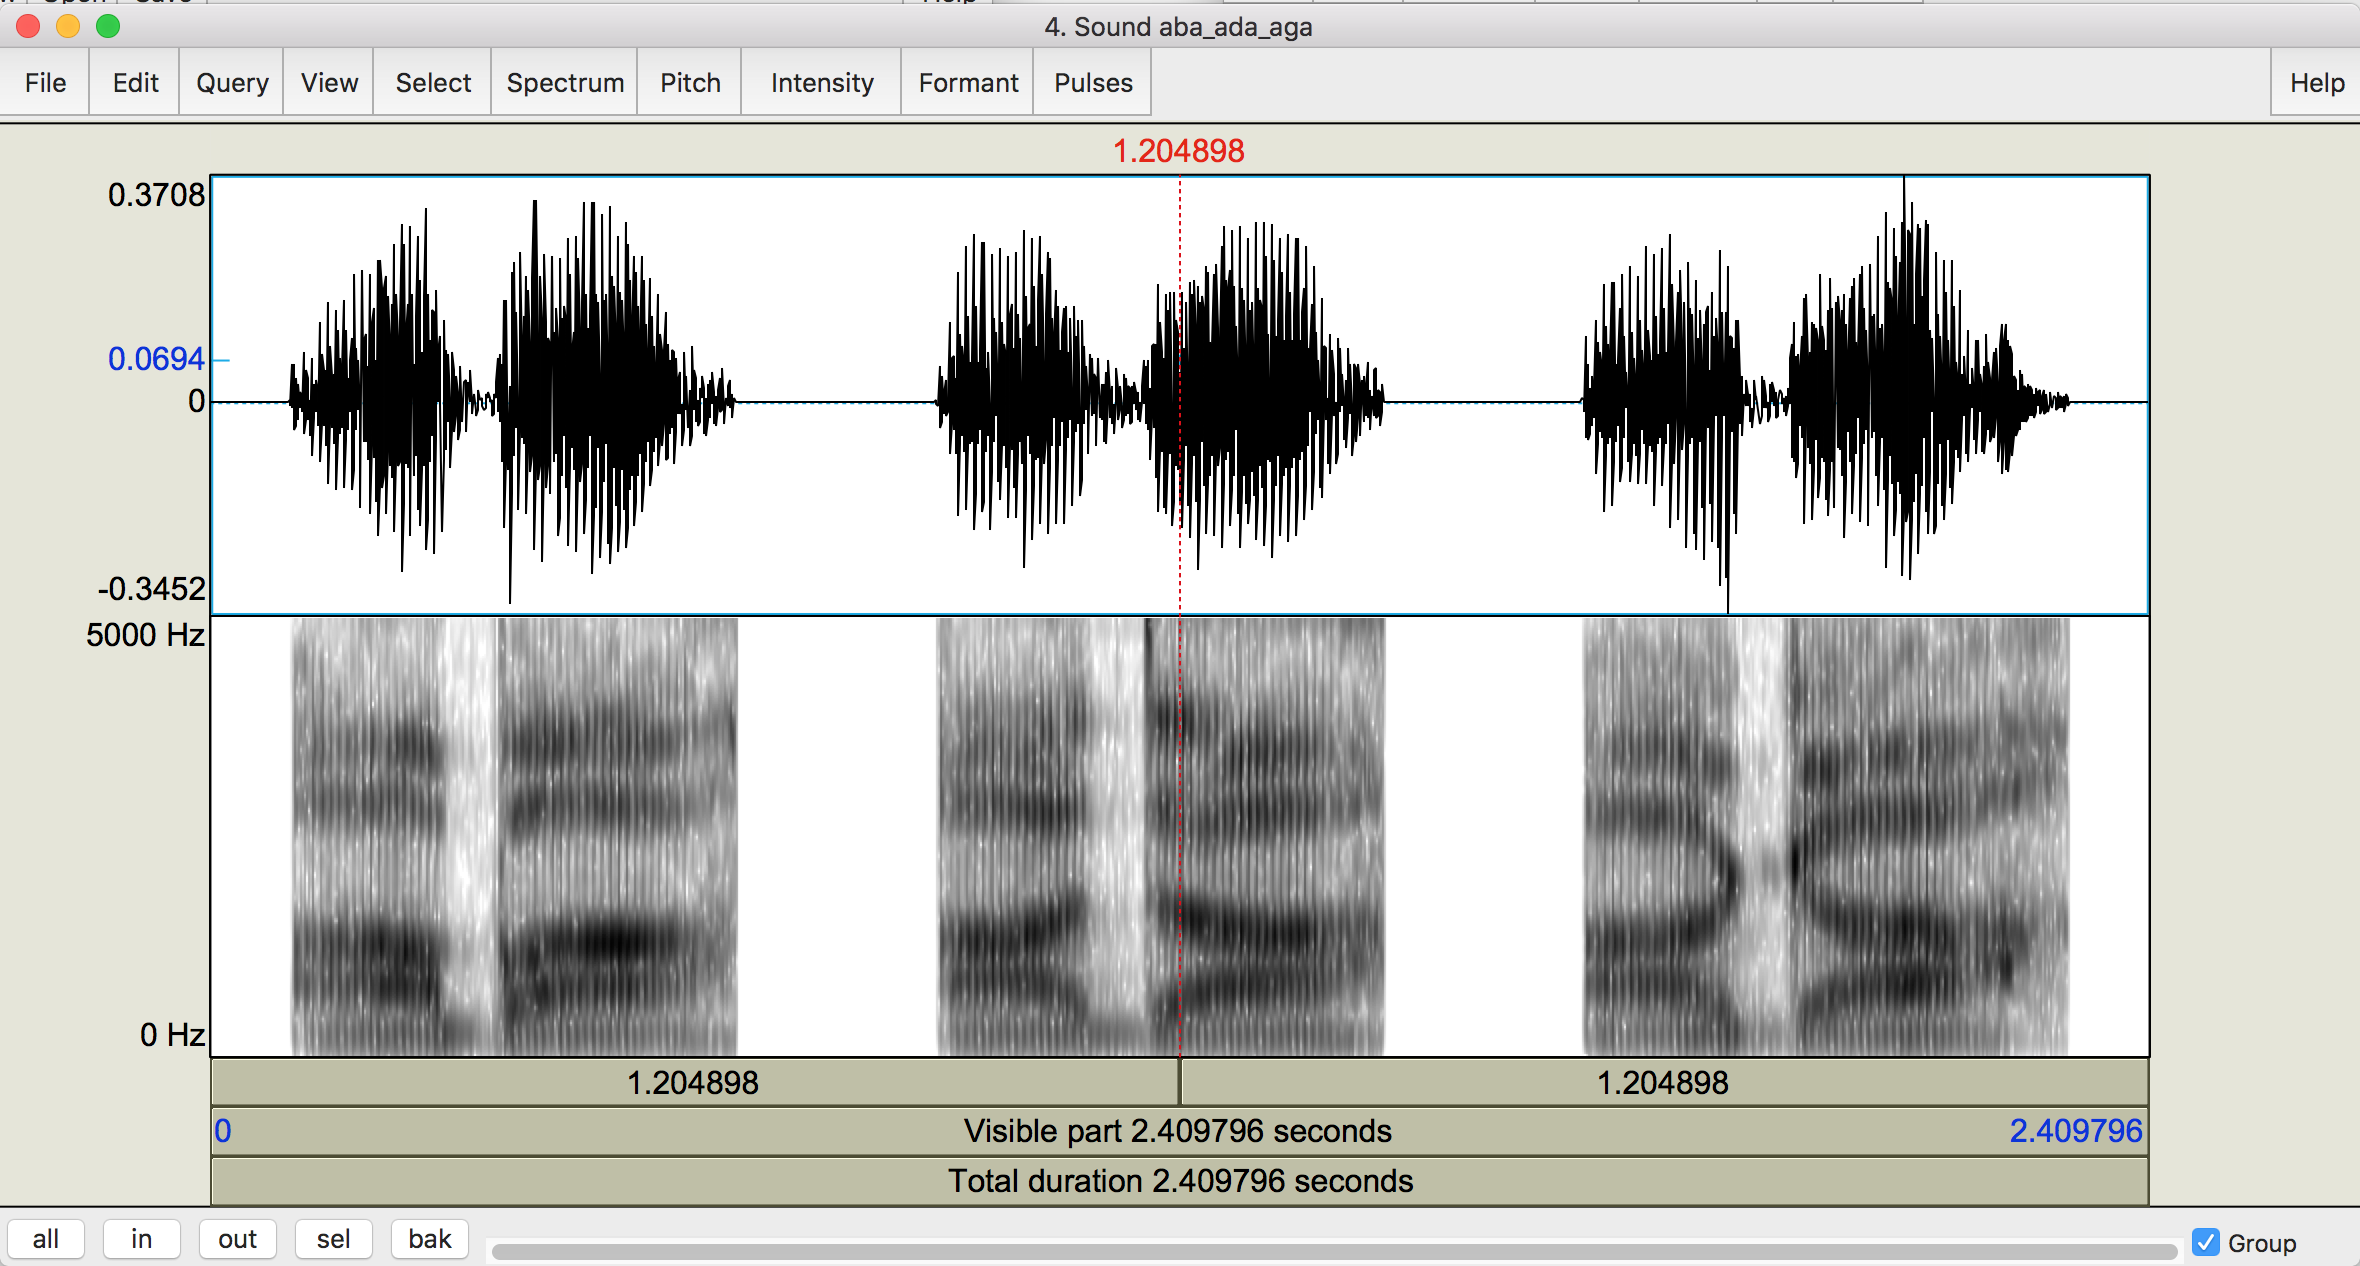
\includegraphics[width=0.8\textwidth]{./figures/Praat_B-01-aba-ada-aga}
	\end{center}
\end{figure}

\paragraph{Write--up:} Once you have the triplet of utterances optimally displayed in front of you (i.e., no red dots indicating the automatic formant tracks), try to figure out what the differences between the consonants are. What looks different in each spectrogram? Does the pattern of formants change according to the consonants you see uttered? What about the shape of individual formants? Try to characterize as best as you can the differences you see. Do you think you can, at least tentatively, characterize the different consonants? That is, do you think you can come up with an acoustic definition of what [b] [d] and [g] are?

Remember to save a picture of your display\footnote{If you do not know how to do that, google ``Print Screen'' or ``Screen capture'' together with your operating system name. In case you want to edit (cropping, for instance) the image you captured, you'll have to use an image editor.} and put it in your write up, so I can see what you saw. Once you have a tentative acoustic definition of each consonant, move on to the next comparison.

\subsubsection{ibi idi igi}

Do the same thing you did for the previous file, but now based on the file \emph{ibi\_idi\_igi.wav}.

\paragraph{Write--up:} Compare the three utterances. What are the differences between the syllables starting with the different consonants? Are they consistent with the ones you observed for the first triplet? What about the tentative acoustic definitions for the consonants you derived from the previous triplet, do they hold for this new series of syllables? Remember to save a picture and put it on your write up. Once you have finished this comparison and written it up, move on to the next one.

\subsubsection{ubu udu ugu}

Do the same thing you did for the previous two files, but now based on the file \emph{ubu\_udu\_ugu.wav}.

\paragraph{Write--up:} Compare the three syllables starting with different consonants. What are the differences between them? Are they consistent with the ones you observed for the first and/or second triplet? What about the tentative acoustic definition for the consonants you derived from the previous triplets, does it hold for this new series of syllables? Remember to save a picture and put it on your write up. Once you have finished this comparison and written it up, move on to the next one.

\subsubsection{idi ada udu}

Do the same thing you did for the previous three files, but now based on the file \emph{idi\_ada\_udu.wav}.

\paragraph{Write--up:} Compare the three syllables that now, unlike the other cases, \emph{start with the same consonant}. Instead of having three different consonants and trying to characterize the differences between them, we are looking at the same consonant; therefore you should try to characterize the similarities between the graphs. By now, you have seen spectrograms for different syllables starting with [d]. Have they been consistent so far? Pay close attention at the shape of the formants. What consequences do you think this has for our ``one--to--one mapping'' hypothesis? Remember to save a picture and put it on your write up. Once you have finished this comparison and written it up, you can move to the final part of the lab.

\subsection{What you need to write up}

All the parts marked as \emph{Write--up} in the instructions above should be incorporated in your lab write--up, together with any plots that may be required. Try to articulate your impressions and results the best you can, in full coherent sentences (no bullets, please).

